\documentclass[border=5pt]{standalone}
\usepackage[UTF8]{ctex}
\usepackage{amsmath}
\usepackage{tikz}
\usetikzlibrary{positioning, arrows.meta, calc}

\begin{document}
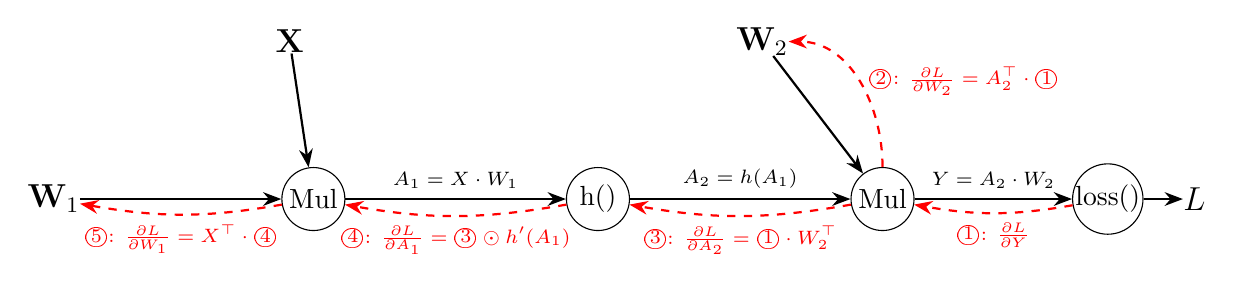
\begin{tikzpicture}[
    node distance=2cm,
    every node/.style={align=center},
    op/.style={circle, draw, minimum size=0.8cm, inner sep=0pt},
    input/.style={inner sep=0pt, font=\large},
    fwdarrow/.style={-Stealth, thick},
    bkarrow/.style={-Stealth, thick, red, dashed},
    label/.style={font=\scriptsize}
]

% 输入节点
\node[input] (X) at (0, 2) {$\mathbf{X}$};
\node[input] (W1) at (-3,0) {$\mathbf{W}_1$};
\node[input] (W2) at (6, 2) {$\mathbf{W}_2$};

% 操作节点
\node[op] (Mul1) at (0.3, 0) {Mul};
\node[op, right=2.8cm of Mul1] (h) {h()};
\node[op, right=2.8cm of h] (Mul2) {Mul};
\node[op, right=2cm of Mul2] (g) {loss()};

% 输出
\node[input, right=0.5cm of g] (L) {$L$};

% 前向传播
\draw[fwdarrow] (X) -- (Mul1);
\draw[fwdarrow] (W1) -- (Mul1);
\draw[fwdarrow] (Mul1) -- node[above, label] {$A_1 = X \cdot W_1$} (h);
\draw[fwdarrow] (h) -- node[above, label] {$A_2 = h(A_1)$} (Mul2);
\draw[fwdarrow] (W2) -- (Mul2);
\draw[fwdarrow] (Mul2) -- node[above, label] {$Y = A_2 \cdot W_2$} (g);
\draw[fwdarrow] (g) -- (L);

% 反向传播
% ①: ∂L/∂Y
\draw[bkarrow] (g) to[out=-170,in=-10] node[below, label] {\textcircled{\scriptsize 1}: $\textstyle \frac{\partial L}{\partial Y}$} (Mul2);

% ②: ∂L/∂W₂
\draw[bkarrow] (Mul2) to[out=90,in=0] node[right, label] {\textcircled{\scriptsize 2}: $\textstyle \frac{\partial L}{\partial W_2} = A_2^\top \cdot \text{\textcircled{\scriptsize 1}}$} (W2);

% ③: ∂L/∂A₂
\draw[bkarrow] (Mul2) to[out=-170,in=-10] node[below, label] {\textcircled{\scriptsize 3}: $\textstyle \frac{\partial L}{\partial A_2} = \text{\textcircled{\scriptsize 1}} \cdot W_2^\top$} (h);

% ④: ∂L/∂A₁
\draw[bkarrow] (h) to[out=-170,in=-10] node[below, label] {\textcircled{\scriptsize 4}: $\textstyle \frac{\partial L}{\partial A_1} = \text{\textcircled{\scriptsize 3}} \odot h'(A_1)$} (Mul1);

% ⑤: ∂L/∂W₁ - 关键修改:使用弯曲路径避免重合
\draw[bkarrow] (Mul1) to[out=-170,in=-10] node[below, label] {\textcircled{\scriptsize 5}: $\textstyle \frac{\partial L}{\partial W_1} = X^\top \cdot \text{\textcircled{\scriptsize 4}}$} (W1);

\end{tikzpicture}
\end{document}